\documentclass[xcolor=pdftex,dvipsnames,table]{beamer}
\usepackage{subfigure}
\usepackage{amsbsy}
\usepackage{tikz}
\usetikzlibrary{arrows}
\usepackage{amsmath,graphicx,dsfont,color}
\usepackage{amsfonts}
\usepackage{amssymb}
\usepackage{array}

\bibliographystyle{apalike}

\setbeamertemplate{bibliography item}{\insertbiblabel}
\setbeamertemplate{bibliography entry title}{}
\setbeamertemplate{bibliography entry location}{}
\setbeamertemplate{bibliography entry note}{}

%Definitiona

\newcommand{\x}{\mathbf{x}}
\newcommand{\X}{\mathbf{X}}
\newcommand{\W}{\mathbf{W}} %Weight
\newcommand{\bais}{\mathbf{b}}%Bais
\newcommand{\act}{\texttt{g}}%Activation
\newcommand{\loss}{L}
\newcommand{\pdata}{\hat{p}_{\texttt{data}}}
\newcommand{\nsize}{n}
\newcommand{\param}{\boldsymbol{\theta}}
\newcommand{\featmap}{\boldsymbol{\phi}}
\newcommand{\EV}{\mathbb{E}}







\usepackage{physics}

\title{Backpropagation}
\author{E. Decencière}
\date{MINES ParisTech}
%To include LOGO?
%\logo{\includegraphics[width=.1\columnwidth]{MinesLogo}}
\useinnertheme{rounded}
\usecolortheme{rose}

\begin{document}
\begin{frame}
\titlepage
\end{frame}

%%%%%%%%%%%%%
\begin{frame}{Backpropagation through a fully connected layer}
\begin{figure}
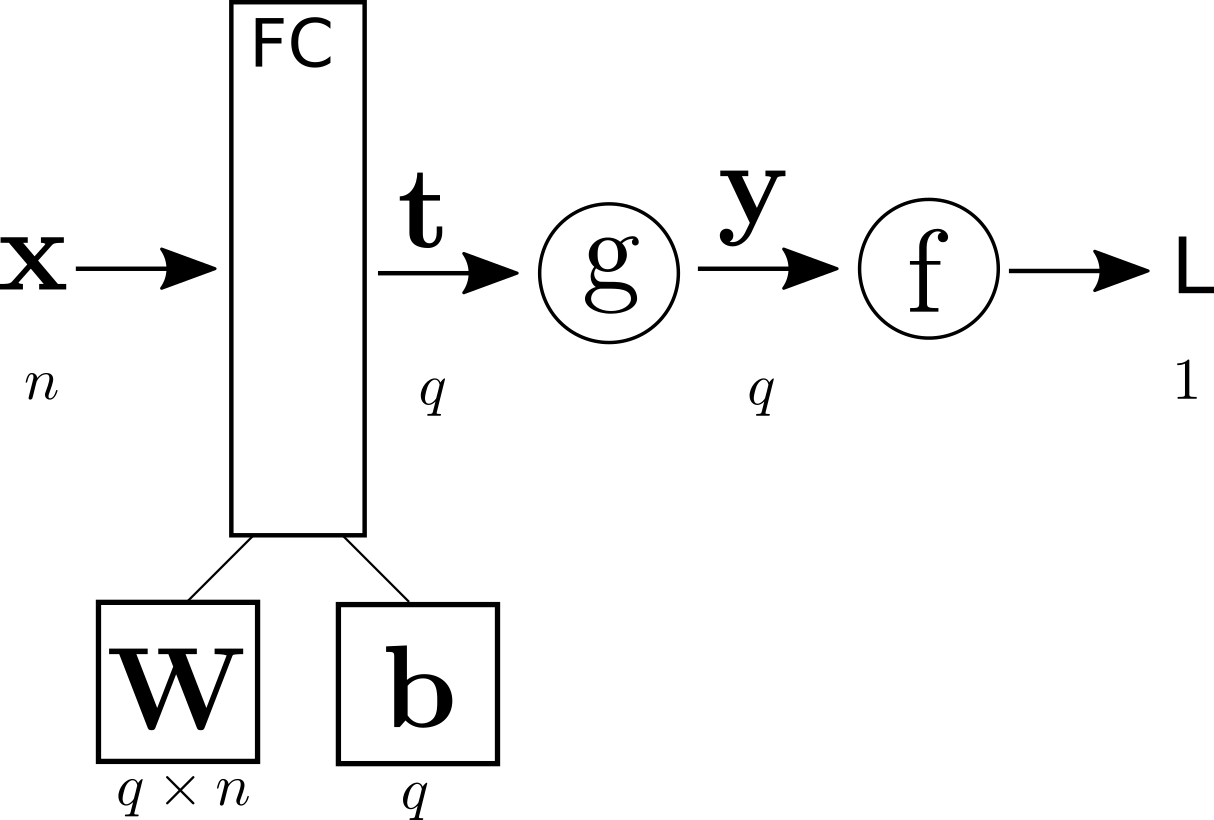
\includegraphics[width=0.5\textwidth]{../graphics/bp_fc.png}
\end{figure}

Setup:
\begin{eqnarray*}
n, q \in \N^*\\
\x \in \R^n \\
\W \in \R^q \times \R^n \\
\bias, \mathbf{t}, \y \in \R^q \\
\loss \in \R
\end{eqnarray*}

\end{frame}

%%%%%%%%%%%%%
\begin{frame}{Backpropagation through a fully connected layer}
\begin{figure}
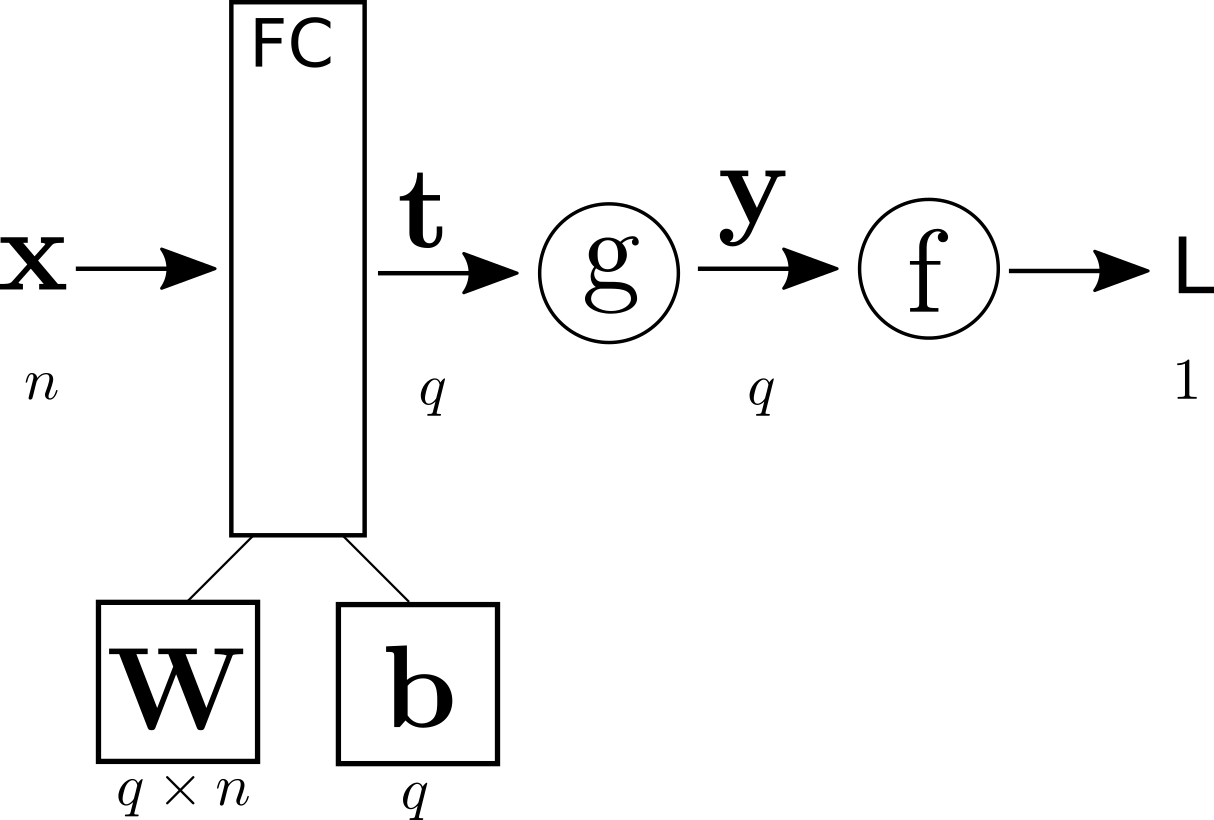
\includegraphics[width=0.5\textwidth]{../graphics/bp_fc.png}
\end{figure}

\begin{columns}
  \begin{column}{0.5\textwidth}
    Forward pass:
    \begin{eqnarray*}
      \mathbf{t} &=& \W\x + \bias \\
      \y &=& \act(\W\x + \bias) \\
      \loss &=& f(\y)
    \end{eqnarray*}
  \end{column}

  \begin{column}{0.5\textwidth}
    Local gradients:
    \begin{eqnarray*}
      \pdv{\mathbf{t}}{\W} &=& \x^t \\
      \pdv{\mathbf{t}}{\bias} &=& 1 \\
      \pdv{\y}{\mathbf{t}} &=& \act'
    \end{eqnarray*}
  \end{column}
\end{columns}

\end{frame}

%%%%%%%%%%%%%
\begin{frame}{Backpropagation through a fully connected layer}
  \begin{figure}
    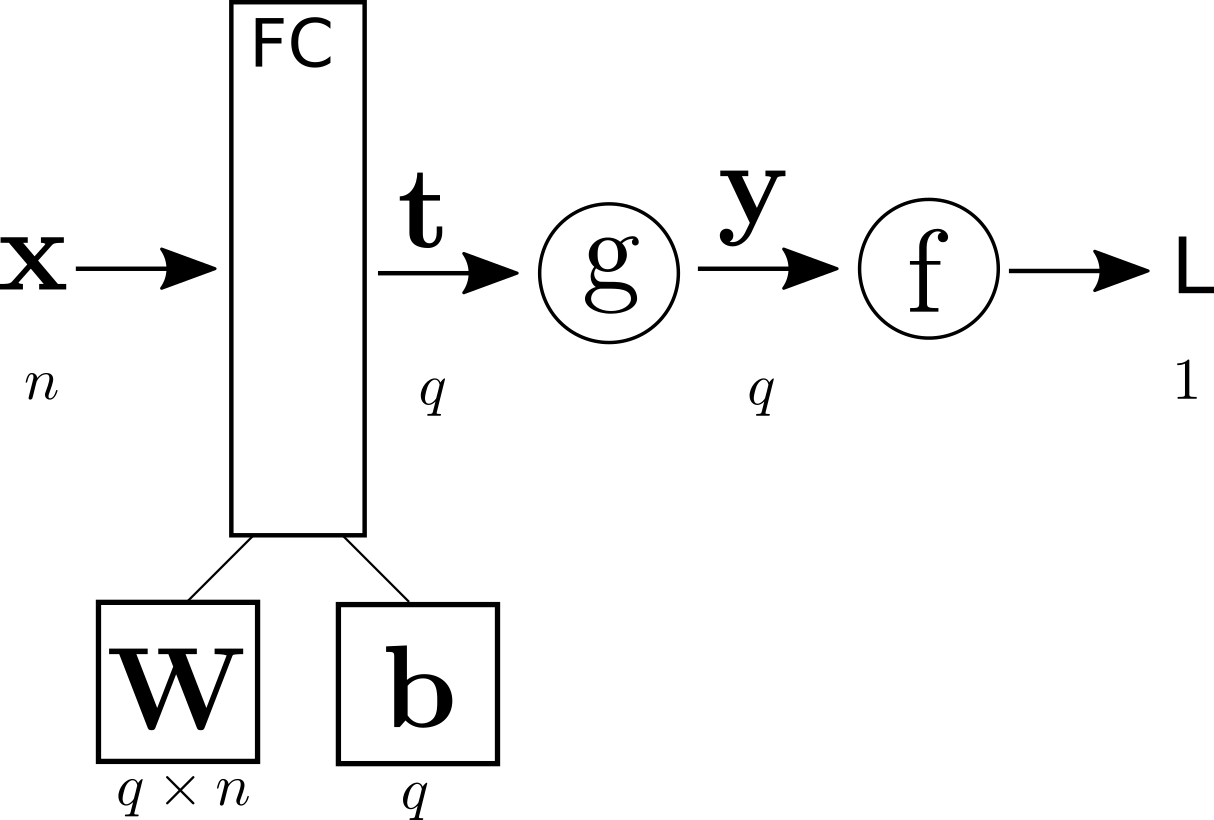
\includegraphics[width=0.5\textwidth]{../graphics/bp_fc.png}
  \end{figure}

  Backpropagation:
  \begin{eqnarray*}
    \pdv{\loss}{\mathbf{t}} &=& \pdv{\loss}{\y}.\pdv{\y}{\mathbf{t}} \\
                           &=& \pdv{\loss}{\y} \odot \act'(\mathbf{t}) \\
  \end{eqnarray*}

\end{frame}

%%%%%%%%%%%%%
\begin{frame}{Backpropagation through a fully connected layer}
  \begin{figure}
    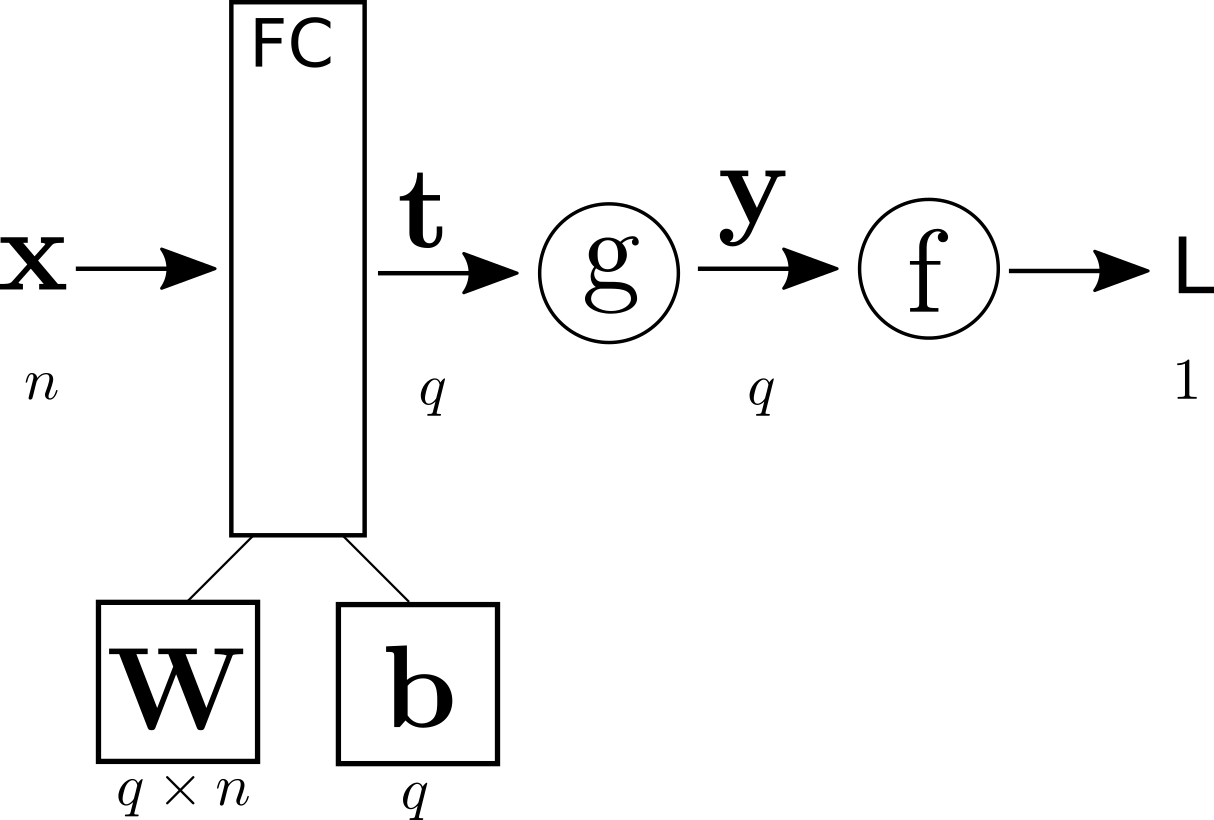
\includegraphics[width=0.5\textwidth]{../graphics/bp_fc.png}
  \end{figure}

  Backpropagation:
  \begin{columns}
    \begin{column}{.5\textwidth}
      \begin{eqnarray*}
        \pdv{\loss}{\W} &=& \pdv{\loss}{\mathbf{t}}.\pdv{\mathbf{t}}{\W} \\
                   &=& \pdv{\loss}{\y} \odot \act'(\mathbf{t}).\x^t
      \end{eqnarray*}
    \end{column}

  \begin{column}{.5\textwidth}
  \begin{eqnarray*}
    \pdv{\loss}{\bias} &=&  \pdv{\loss}{\y} \odot \act'(\mathbf{t})
  \end{eqnarray*}
  \end{column}
\end{columns}


\end{frame}

\end{document}
